\section{Required laser power}\label{ssec:HDM_required_laser_power} The laser power too requires new calculations when compared to those performed in \cref{ssec:required_laser_power}. First and foremost, the resolution required for the Hazard Detection Mode is $5\,cm$, with a resulting maximum allowable standard deviation of $\sigma_{tot}=142\,ps$. Finally, it was decided that a scanning method would be used where the target area would be divided into at least $2048/8=256$ pieces. \Cref{fig:hdm_s_vs_n} and \cref{fig:hdm_s_vs_n_small} show the updated relationship between signal and noise photons to meet the requirements.

\begin{figure}[h]
\centering
	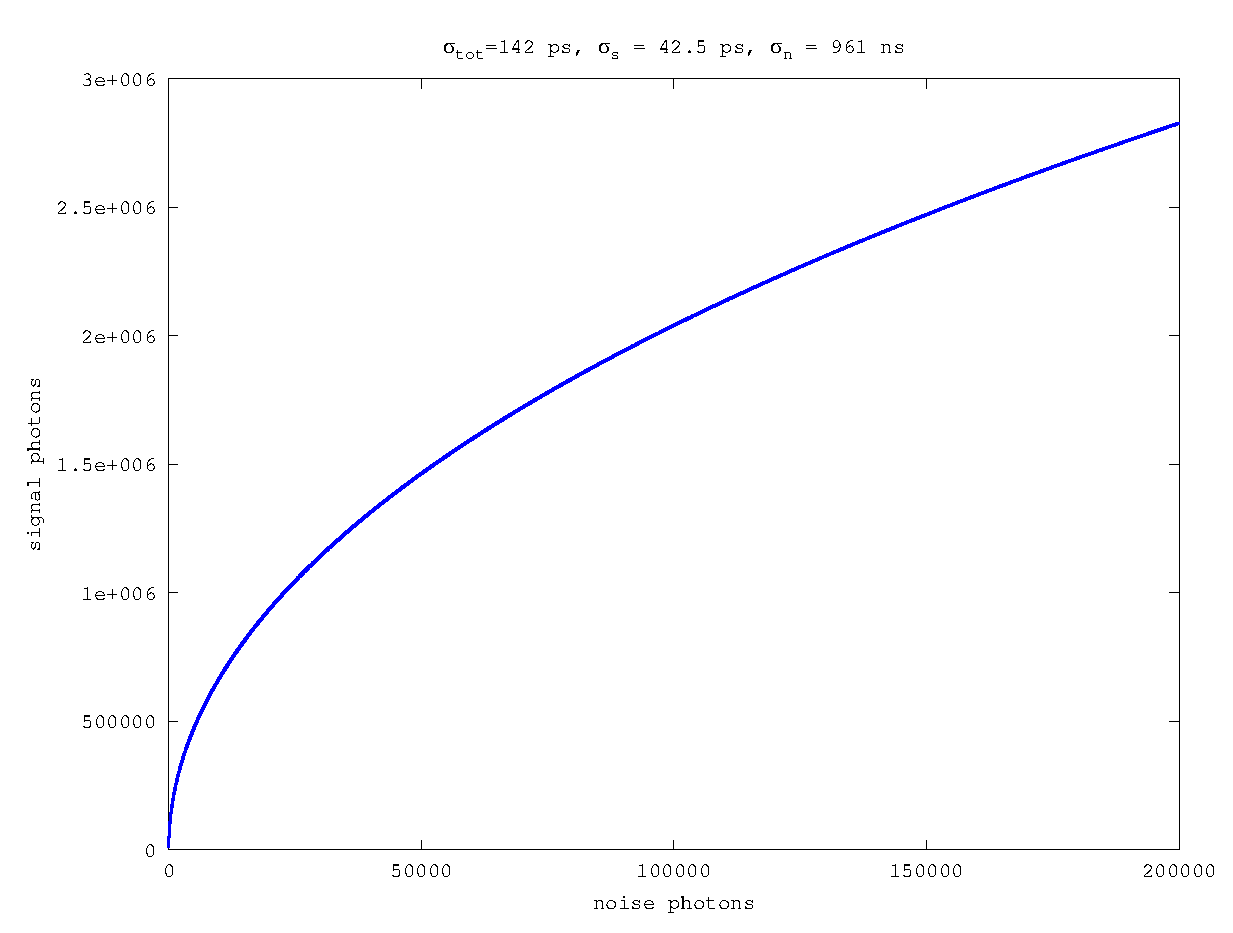
\includegraphics[width=0.8\linewidth]{fig/hdm_s_vs_n.eps}
\caption{required signal photons for a given number of noise photons to meet the HDM requirements at maximum altitude}
\label{fig:hdm_s_vs_n}
\end{figure}

\begin{figure}[h]
\centering
	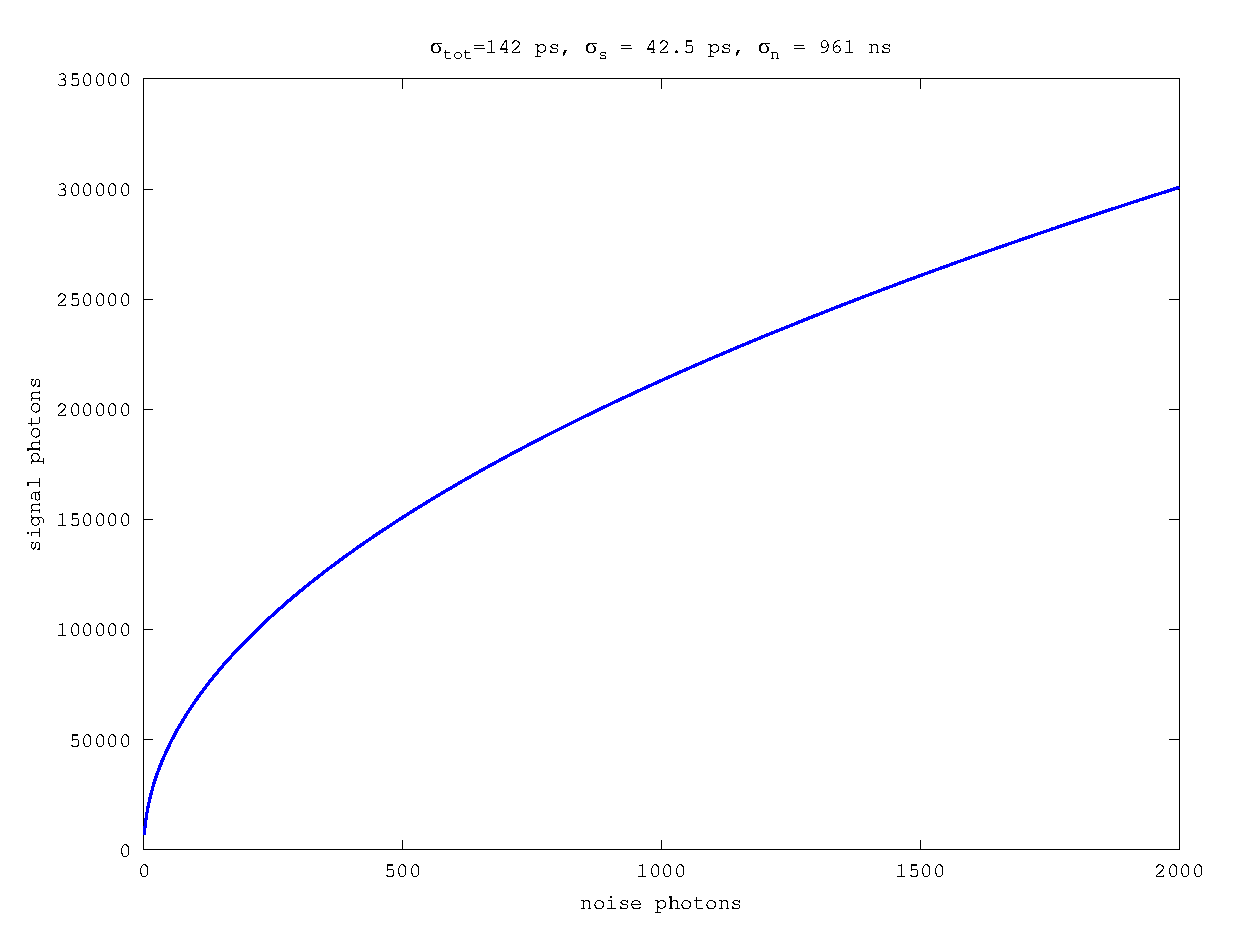
\includegraphics[width=0.8\linewidth]{fig/hdm_s_vs_n_small.eps}
\caption{required signal photons for a given number of noise photons to meet the HDM requirements at maximum altitude}
\label{fig:hdm_s_vs_n_small}
\end{figure}

All the acquired new information can now be used to calculate a new relationship between the required peak power and average power. Note that in this case the least amount of pulses is 256. The reason being oly a 1/256th of the target can be observed at a time. The results of these calculations are shown in \cref{fig:hdm_peak_vs_av}. This time increasing the number of pulses does decrease the required signal power significantly. The more important result is however, that the power budget is orders of magnitude of for obtaining a feasible peak optical power for the laser. Therefore the HDM modus is not feasible without extra processing like an energy threshold.

\begin{figure}[h]
\centering
	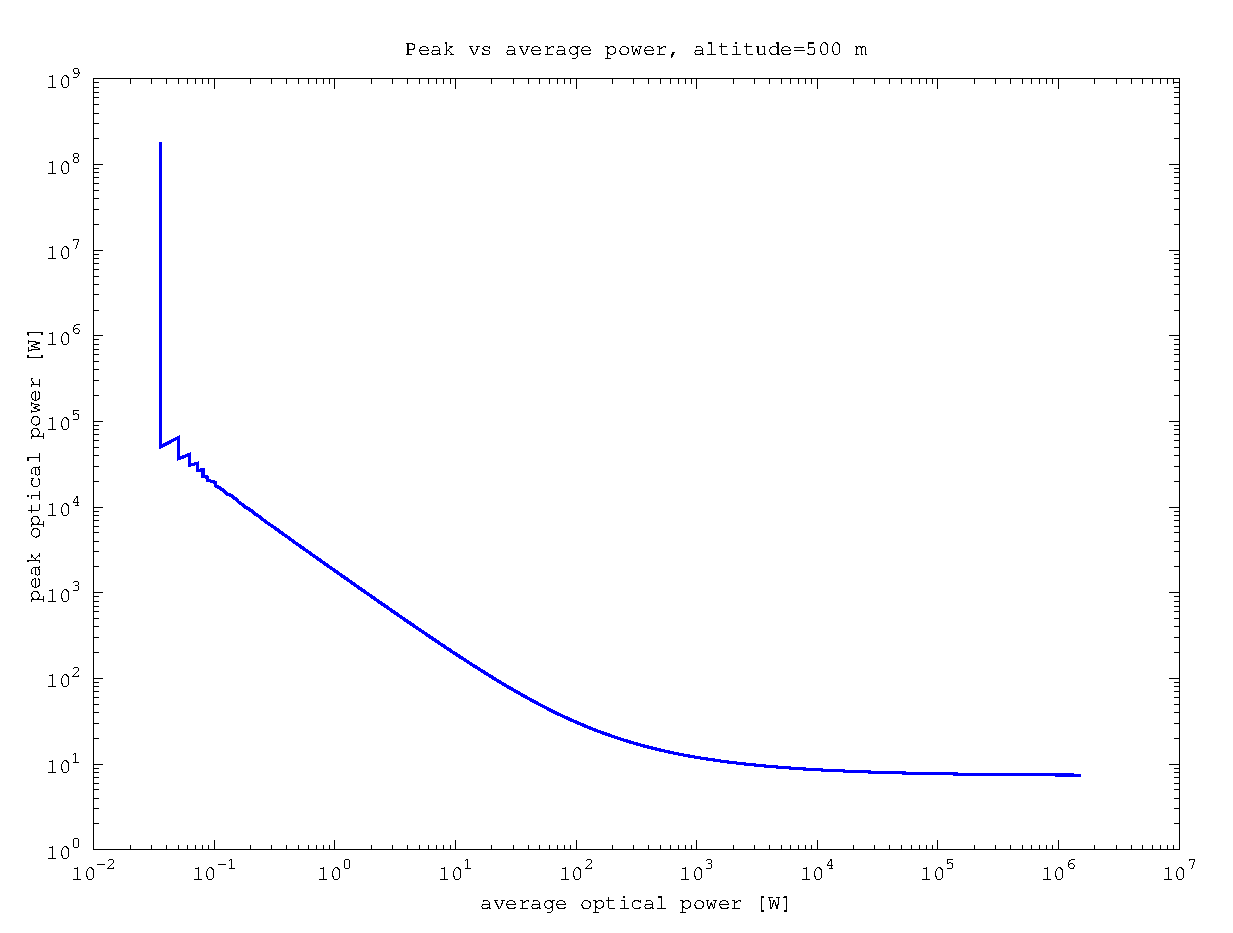
\includegraphics[width=0.8\linewidth]{fig/hdm_peak_vs_av.eps}
\caption{required signal photons for a given number of noise photons to meet the HDM requirements at maximum altitude}
\label{fig:hdm_peak_vs_av}
\end{figure}

The next step is to look at the energy threshold again. The average noise power $P_B=7.4\,W$. In order to make sure that the expected amount of photons per bin is 10 times higher than for the noise, one needs a peak power of $P_{peak}=74\,W$. The resulting average optical laser power is calculated below.

\begin{align*}
	P_{av}&=P_{peak}\cdot\frac{2048}{8}\cdot FWHM\\
	&= 74\cdot256\cdot100\cdot10^{-12}\\
	&= 1.89\,\mu W
\end{align*}

Both the peak and average laser power fall royally in the power budget. This means that the device can meet the resolution requirements within the power budget, granted that the damage caused by radiation can be reasonably contained. This will be investigated in \cref{sec:radiation}. Another important, but less pressing challenge is the design of the readout and the data processing of the SPAD array. 
